%%%%%%%%%%%%%%%%%%%%%%%%%%%%%%%%%%%%%%%%%
% Stylish Article
% LaTeX Template
% Version 2.1 (1/10/15)
%
% This template has been downloaded from:
% http://www.LaTeXTemplates.com
%
% Original author:
% Mathias Legrand (legrand.mathias@gmail.com) 
% With extensive modifications by:
% Vel (vel@latextemplates.com)
%
% License:
% CC BY-NC-SA 3.0 (http://creativecommons.org/licenses/by-nc-sa/3.0/)
%1
%%%%%%%%%%%%%%%%%%%%%%%%%%%%%%%%%%%%%%%%%

%--------------------------------------------------------------# Path to your oh-my-zsh installation.--------------------------
%	PACKAGES AND OTHER DOCUMENT CONFIGURATIONS
%----------------------------------------------------------------------------------------

\documentclass[fleqn,10pt]{SelfArx} % Document font size and equations flushed left

\usepackage[english]{babel} % Specify a different language here - english by default

\usepackage{marvosym, epigraph, subfig, listings}

\usepackage[sortcites=false,style=authoryear-comp,bibencoding=utf8, natbib=true, firstinits=true, maxcitenames=2, maxbibnames = 99, uniquename=false, backend=bibtex, useprefix=true, backref=false,doi=false,isbn=false,url=false,dashed=true]{biblatex}
\setlength\bibhang{20pt}
\bibliography{references.bib}
\AtEveryBibitem{%
	\clearfield{day}%
	\clearfield{month}%
	\clearfield{endday}%
	\clearfield{endmonth}%
}

%----------------------------------------------------------------------------------------
%	COLUMNS
%----------------------------------------------------------------------------------------

\setlength{\columnsep}{0.55cm} % Distance between the two columns of text
\setlength{\fboxrule}{0.75pt} % Width of the border around the abstract

%----------------------------------------------------------------------------------------
%	COLORS
%----------------------------------------------------------------------------------------

\definecolor{color1}{RGB}{0,0,90} % Color of the article title and sections
\definecolor{color2}{RGB}{0,20,20} % Color of the boxes behind the abstract and headings

%----------------------------------------------------------------------------------------
%	HYPERLINKS
%----------------------------------------------------------------------------------------

\usepackage{hyperref} % Required for hyperlinks
\hypersetup{hidelinks,colorlinks,breaklinks=true,urlcolor=color2,citecolor=color1,linkcolor=color1,bookmarksopen=false,pdftitle={What drives which region?},pdfauthor={Thomas de Graaff}}

%----------------------------------------------------------------------------------------
%	ARTICLE INFORMATION
%----------------------------------------------------------------------------------------

\JournalInfo{Conference paper} % Journal information 
\Archive{Prepared for ERSA 2019} % Additional notes (e.g. copyright, DOI, review/research article)

\PaperTitle{Housing market and migration revisited: a multilevel gravity model for Dutch municipalities}

\Authors{Thomas de Graaff\textsuperscript{1}*} % Authors
\affiliation{\textsuperscript{1}\textit{Department of Spatial Economics, Vrije Universiteit Amsterdam, Amsterdam, The Netherlands}} % Author affiliation
\affiliation{*\textbf{Corresponding author}: \Letter{} t.de.graaff@vu.n; \Mundus{} \href{thomasdegraaff.nl}{thomasdegraaff.nl}} % Corresponding author

\Keywords{Gravity model --- housing market --- migration --- multilevel model --- partial pooling --- prediction}
\newcommand{\keywordname}{Keywords} 

%%----------------------------------------------------------------------------------------
%%	ABSTRACT
%%----------------------------------------------------------------------------------------

\Abstract{This paper revisits the impact of the housing market
  structure on interregional migration, but adopts an alternative
  modeling approach to migration flows between cities. The starting
  point is a gravity model, but instead of using fixed effects for
  cities of origin and destination, I use a multilevel mixed effects
  approach allowing me to simultaneously model migration flow
  characteristics and the cities of origin and destination
  characteristics. This approach has two main advantages. First, it
  allows for simultaneous estimation of the impact of city
  characteristics on migration flows, where the impact is not
  necessarily symmetrical for cities of origin and
  destination. Second, it allows for prediction of migration flows
  between cities both in and out of sample. Preliminary results show
  that homeownership decrease migration flows significantly with an
  elasticity below $-1$. Municipal social renting rate has a negative
  impact as well, but its elasticity is close to zero.}

%----------------------------------------------------------------------------------------
\hypersetup{draft} 
\begin{document}
	
	\flushbottom % Makes all text pages the same height
	\maketitle % Print the title and abstract box
	%\tableofcontents % Print the contents section
	\thispagestyle{empty} % Removes page numbering from the first page
	
	%----------------------------------------------------------------------------------------
	
	\section{Introduction} % The \section*{} command stops section numbering

        In the 1990s, Andrew Oswald wrote two famous working papers
        \citep{oswald1996conjecture, oswald1999housing} postulating
        that homeownership rates would have a negative impact on labor
        market behavior, as the high costs of moving residence
        associated with homeownership would impede regional
        mobility. These two working papers evoked a large empirical
        literature \citep[see, e.g., ][]{munch2006homeowners,
          munch2008home, de2013european} looking at the impact of
        individual and aggregate homeownership on labor market
        performance, where seemingly paradoxically at the aggregate
        level homeownership is indeed harmful for labor market
        behavior where at the individual level it is correlated with
        positive labor market performance.

        That housing market structure has an effect on migration
        decisions is well-established, especially at the micro-level,
        where it is widely accepted that homeownership has a negative
        effect on regional mobility \citep{dietz2003social}. For
        example, \citet{palomares2018understanding} find that
        homeownership has a very strong immobility effect on in
        internal migration in Spain during the period 2001--2011.

        On an aggregate level, \citet{amirault2016drags} already
        looked at the impact of homeownership on migration flows
        within a gravity model using a Poisson pseudo maximum
        likelihood estimator and found an elasticity around
        $-1$. However, traditional gravity modeling has the
        disadvantage that either regional fixed effects of origins and
        destinations can be incorporated or the regions'
        characteristics when not varying over flows. Moreover,
        theoretically, regional effecs should be incorporated leaving
        no room in the traditional approach to incorporate regional characteristics

        This paper circumvents this disadvanted by adopting a
        multilevel approach with partial pooling\footnote{There is a
          whole variety of names for these types of models, including
          varying effects, mixed effects and shrinkage models. I use
          the more generic multilevel description as regions and flows
          are by definition measured at a different level (scale).},
        where the latter terms indicates that I adopt regions of
        origin and destination specific effects, but that I ``draw''
        them from a distribution, hence the name partial pooling
        (where complete pooling states no group effects and no pooling
        fixed effects.

        A partial pooling approach has another advantege, namely the
        regional specific effects are completely probabilistic, making
        it feasible to predict both within and out-of-sample. In other
        words, with the results at hand I can predict flows between
        hypothetical regions.

        This paper reads as follows. The next section describes the
        data and focuses especially on the distribution of regional
        migration flows and regional labour market structure. Section
        3 describes the modeling approach, where starting from
        traditional gravity model and using the descriptives of
        migration flows I argue for a specific type of model. Section
        4. gives both the model results and their analysis. By the
        latter I mean that this sections deals as well with
        interpretation by giving prediction both within and
        out-of-sample. The last section concludes.

        \section{Data}

              \begin{figure*}[ht!]\centering % Using \begin{figure*} makes the figure take up the entire width of the page
          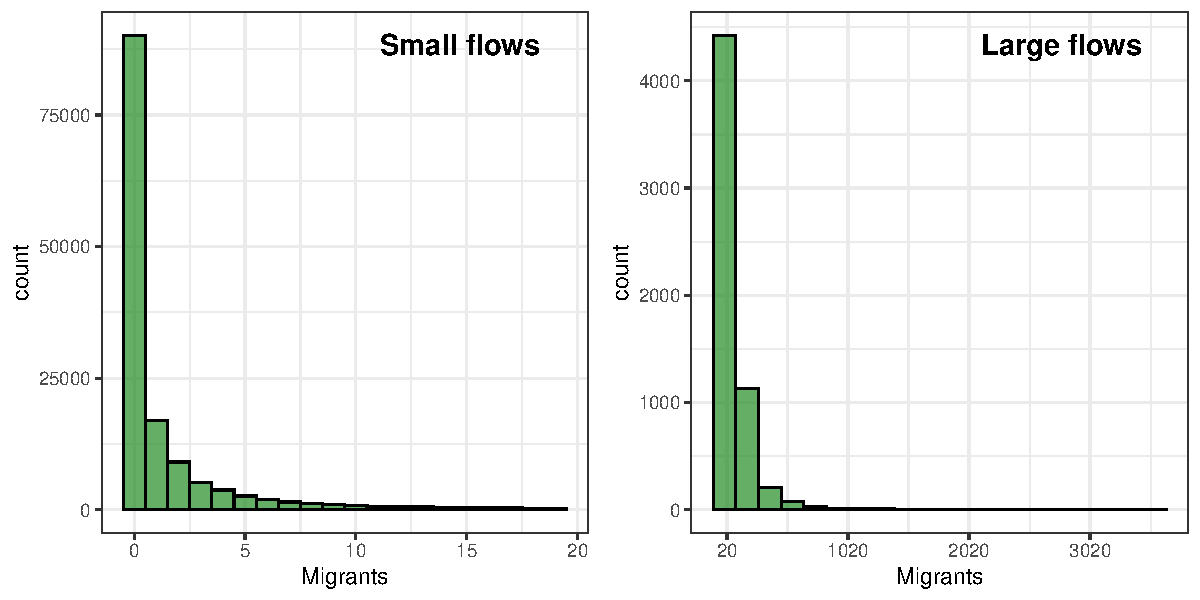
\includegraphics[width=0.8\linewidth]{../fig/hist_mig.pdf}
          \caption{Histogram of migrant flows. Left panel shows the
            histogram of small migrant flows ($N<0$) and the right
            panel shows the histogram of large migrant flows
            ($N \geq 20$). Note the different scale of the y-axis.}
          \label{fig:hist_mig}
        \end{figure*}

        I model the migration flows measured in individuals between
        the 393 Dutch municipalities in 2015. There is no information
        available about within municipality residential migration. So,
        I have 393 regional characteristics (or doubled when
        accounting for both regions of origin and destination) and
        154,056 flows ($393 \times 393 - 393$). 

        Figure \ref{fig:hist_mig} shows the distribution of migrant
        flows within my sample. The left panel deals with migrant
        flows below 20, the right panel with migrant of 20 and
        larger. Two main observations can be made.

        First, there is strong but consistent decay in both panels,
        which points to a strong underlying pattern. However, the
        `tail' in this distribution is rather thick.\footnote{The
          largest migration flows are between the municipalities of
          Amsterdam and Amstelveen and amount to about 3,500
          migrants.} There are still observations quite far right in
        the distributution. Indeed, sample mean is about 10, while the
        sample variance is aournd 40, leading to a strong presence of
        \emph{overdispersion}.

        Secondly, most of my dataset consists of zero
        observations. Although they do seem to be genuine observations
        and not caused by another proces (we will check for this
        later), they do need to be taken specifically into account. 

        I include 7 other variables in my model. First, to account for
        spatial distance decay between origin $i$ and destination $j$,
        distance between all municipalities are calculated as
        Eucledian distance between centroids
        ($\text{dist}_{ij}$). Secondly, as municipality mass we use
        population size (so $\text{pop}_i$ and
        $\text{pop}_j$). Finally, for housing market structure we use
        variables indicating percentage of homeownership
        ($\text{home}_i$ and $\text{home}_j$ and percentage of social
        renting ($text{soc}_i$ and $\text{soc}_j$). Social renting in
        the Netherlands includes all kinds of renting but typically
        involves local housing corporations offering housing to lower
        income households, where eligibility is based on (lcoal) waiting
        lists. Both social renting and homeownership are assumed to
        impede regional mobility \citep{de2009homeownership}.

        \begin{figure*}[ht]\centering % Using \begin{figure*} makes the figure take up the entire width of the page
          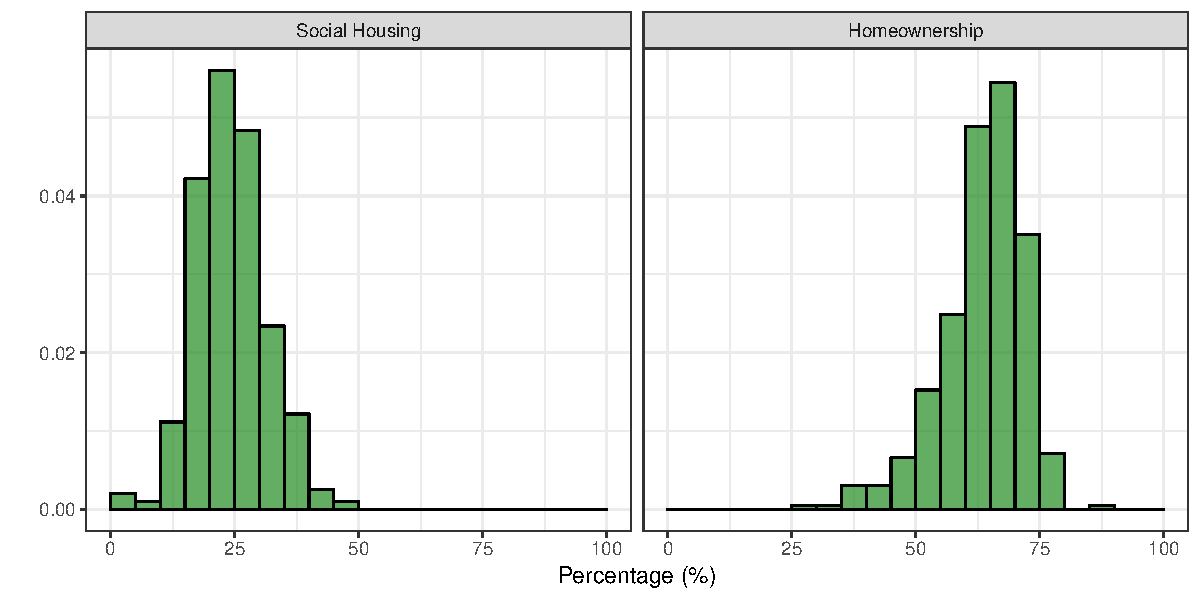
\includegraphics[width=0.8\linewidth]{../fig/hist_housing.pdf}
          \caption{Histogram of social housing (left) and
            homeownership (right) percentages in Dutch municipalities
            2015}
            \label{fig:housing_mig}
        \end{figure*}

        Figure \ref{fig:housing_mig} shows the distribution of social
        renting and homeownership across Dutch municipalities in 2015.
        Clearly, both types of homewnership are important for the
        Netherlands, with an average of 25\% of social housing and
        around 60\% of homeownership. Moreover, it is worthwhile to
        note that social renting is especially prevalent in the the
        larger cities (e.g., Amsterdam has about 40\% social renting
        rate). Also, some smaller dutch municipalities do not exhibit
        any social renting.
        
        \section{Modeling framework}

        \subsection{The traditional gravity model}

        We adopt the basic gravity model specification pioneered by
        \citet{tinbergen1962shaping}, so:
        \begin{equation}
          \text{migrants}_{ij} = \text{pop}_i^{\beta_1}\text{pop}_j^{\beta_2}\text{dist}_{ij}^\gamma
          \label{eq:grav}
        \end{equation}
        Note, that in model (\ref{eq:grav}) the variable
        $\text{dist}_{ij}$ may inhibit all sorts of frictions, not
        only physical distance. Thus, in my case we incorporate
        variables for homeownership and social renting to account for
        frictions on the housing market that may impede regional
        mobility.

        Importantly, \citet{anderson2003gravity} argued that origin
        and destination specific variables should be incorporated to
        take into account multilateral resitance terms. Most oftens,
        this is done by log-linearizing model
        (\ref{eq:grav})\footnote{In our case, note that zeros are
          present in our social renting variable. We therefore add a
          small number to this variables (0.0001). Doing this only on
          the \emph{right-hand side} does not affects our results} and
        incorporating fixed effects for origins and destinations, as
        follows:
        \begin{equation}
          \log(\text{migrants}_{ij}) = o_i + d_j +  \gamma\log(\text{dist}_{ij})
          \label{eq:gravfixed}
        \end{equation} 
        Unfortunately, this approach does not allow for municipality
        specific variables; so, population and housing market
        variables drop out of this model. But those are exactly the
        variables we are interested in! Moreover, equation
        (\ref{eq:gravfixed} is typically estimated with regression
        type of models, which is often very cumbersome given the large
        amount of zeros present flows of migrants.

        Therefore, I next allow for a different strategy, where I
        would like to tackle both the disadvantes of above:
        incorporating both region specific effects and variables and
        modeling the distribution of migrants flows as they are
        displayed in Figure \ref{fig:hist_mig}.

        \subsection{A multilevel gravity model}

        Firstly, as regional migrants flows are discrete and
        relatively rare give the size of the population, the most
        appropriate way to go forward is to model number of migrants
        with a Poisson type of model. However, given that the sampling
        variance is four times the sampling mean of the migration
        flows, we need to correct for overdispersion of
        heteroskedasticity \citep[][states that heteroskedasticity
        (rather than the presence of too many zeros) is responsible
        for the main differences.]{silva2006log}. An often used
        distribution to account for overdispersion is the
        gamma-poisson model (also known as the negative binomial
        model). So, we use that for our outcome variable. 

        To account for the multiplicative nature of the theoretical
        model as in (\ref{eq:grav}), I adopt a log-link for the
        expectation variable in the Poisson model.

        Finally, to adopt both region effects and variables I adopt a
        multilevel model with partial pooling. This entails that our
        regional specific effects (the formerly fixed effecs) are
        drawn from a, in this case Normal, distribution, where the
        parameters of this distrbution are estimated as well (in the
        literature they are known as well as
        hyper-parameters). Intuitively, this entails that regions are
        partially pooled indicating that information between regions
        is shared. This is very attractive, as fixed effects for no
        pooling. The model only learns from the information contained
        in that specific region. The partial pooling also ensures that
        outliers (very high or low effects) are effectively
        \emph{shrunk} towards the mean. Indeed, this is a further
        extension of that best feature of linear regression:
        regression towards the mean.

        The total model looks now as follows:
        
        \begin{subequations}
          \begin{align} \text{Migrants}_{ij} \sim & \text{GammaPoisson}(\lambda_{ij}, \tau) \label{outcome}\\
            \log(\lambda_{ij}) =
            & \alpha + o_{\text{mun}[i]} + d_{\text{mun}[j]} + \notag
            \\ & \beta_1 \log(\text{pop}_i) +
            \beta_2\log(\text{pop}_j) + \notag \\ & \beta_3
            \log(\text{home}_i) + \beta_4 \log(\text{home}_j) + \notag\\
            & \beta_5 \log(\text{soc}_i) + \beta_6 \log(\text{soc}_j)
            + \notag \\ & \beta_7 \log(\text{dist}_{ij}) \label{linear} \\
            o_{\text{mun}} \sim& \text{ Normal}(\alpha_o, \sigma_o) \label{muno} \\
            d_{\text{mun}} \sim& \text{ Normal}(\alpha_d, \sigma_d) \label{mund} \\
            \beta_1,\ldots, \beta_7 \sim& \text{
                                          Normal}(0,2)\\ \alpha_o, \alpha_d \sim& \text{ Normal}(0,2)\\
            \sigma_o, \sigma_d \sim& \text{ HalfCauchy}(0,1) \\ \tau
            \sim& \text{ Gamma}(0.01, 0.01)
          \end{align}
          \label{model}
        \end{subequations}

        The first line ({\ref{outcome}) models the outcome variable,
          being the number of migrants, using a Poisson distribution
          (with parameter $\lambda_{ij}$) allowing for overdispersion
          by using an additional parameter $\tau$. The linear part of
          the model is given by (\ref{linear}) and states that the
          poisson outcome space in on a log-scale and that most
          parameters are on a log-scale as well, allowing for direct
          comparison of the parameters being elasticities. Equations
          (\ref{muno}) and {(\ref{mund}) constitute the multilevel
            part, where parameters $\sigma_o$ and $\sigma_d$ measure
            the amount of pooling. If they tend to zero, there the
            data exhibits complete pooling. If they become very large
            (go to infinity) there is no pooling (thus fixed
            effects). All other parameters are priors (chosen such
            that they are rather conservative but given the amount of
            data they are of little influence).
          
        \section{Results}

        \subsection{Parameter estimates}
        
        I estimated model (\ref{model}) by using the \emph{No U-Turn
          Sampler} (NUTS) in Stan.\footnote{As interface to Stan
          \citep[see for an overview article of
          Stan][]{carpenter2017stan} I used the \texttt{brms}
          R-package \citep{brms}.} NUTS is a relatively recent
        developed Hamiltonian Monte Carlo (a specific form of Markov
        Chain Monte Carlo simulation) method, able to draw samples
        efficiently from large multilevel models
        \citep{hoffman2014no}. Parameter estimates and probability
        intervals of the main parameters (so not the region specific
        effects: there are 786 of them) are given in Table
        \ref{tab:coef}. Perhaps more insightful, there are graphically
        depicted in Figure \ref{fig:forestplot}.

% latex table generated in R 3.4.4 by xtable 1.8-3 package
% Fri Feb 22 15:07:02 2019
\begin{table}[ht]
  \centering
  \caption{Parameter estimates with 95\% probability intervals (group speficic origin and destination estimates are not presented)}
  \label{tab:coef}
  \begin{tabular}{lrrrr}
    \toprule
    Parameter & mean & sd & 2.5\% & 97.5\% \\ 
    \midrule
    b\_Intercept & -0.74 & 0.04 & -0.82 & -0.66 \\ 
    b\_pop\_d & 0.89 & 0.03 & 0.83 & 0.96 \\ 
    b\_pop\_o & 0.88 & 0.04 & 0.79 & 0.97 \\ 
    b\_hom\_d & -1.48 & 0.19 & -1.86 & -1.10 \\ 
    b\_hom\_o & -1.27 & 0.25 & -1.75 & -0.78 \\ 
    b\_soc\_o & -0.04 & 0.04 & -0.11 & 0.03 \\ 
    b\_soc\_d & -0.06 & 0.03 & -0.12 & -0.01 \\ 
    b\_log\_distance & -1.96 & 0.01 & -1.97 & -1.95 \\ 
    sd\_destination\_\_Intercept & 0.45 & 0.02 & 0.42 & 0.49 \\ 
    sd\_origin\_\_Intercept & 0.61 & 0.02 & 0.57 & 0.66 \\ 
    shape & 1.22 & 0.01 & 1.20 & 1.24 \\ 
    \bottomrule
  \end{tabular}
\end{table}

\begin{figure}
  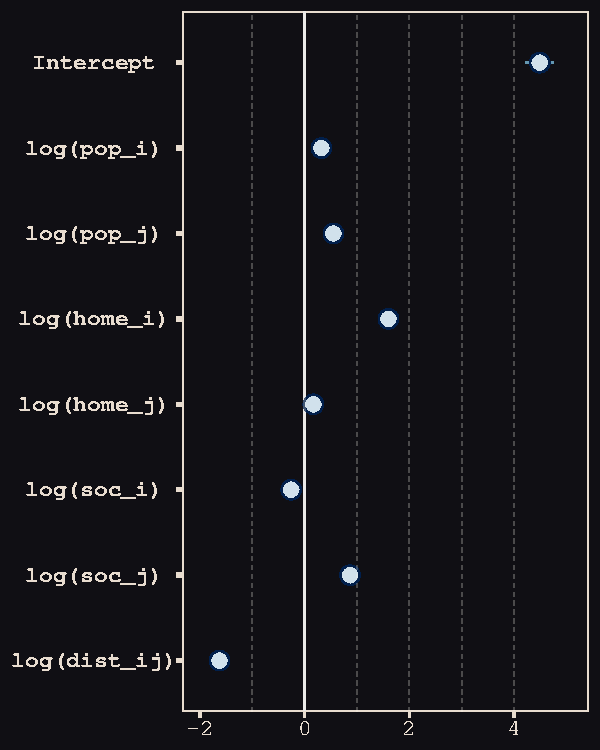
\includegraphics[width = \columnwidth]{../fig/forestplot.pdf}
  \caption{Forest plot of parameter means and 95\% probability
    intervals (group speficic origin and destination estimates are not
    presented)}
  \label{fig:forestplot}
\end{figure}

As most important conclusions in this stage can we say that housing
structure indeed impedes regional mobility, but that it is mainly
homeownership rates and not social renting rates that have a negative
effect. The homeownership elasticities are slightly larger in absolute
size than what \citet{amirault2016drags} reported. Furthermore,
estimations for parameters $\sigma_o$ and $\sigma_d$ point to more
pooling than less, so fixed effects in this case might lead to
substantial overfitting.

\subsection{Model predictions}

\section{In conclusion}

\section*{Acknowledgments} % The \section*{} command stops section numbering

Paper, data and code can be retrieved from the project's GitHub page: \href{https://github.com/Thdegraaff/migration_gravity}{https://github.com/Thdegraaff/migration\_gravity}. 
	%----------------------------------------------------------------------------------------
	%	REFERENCE LIST
	%----------------------------------------------------------------------------------------
	
	\addcontentsline{toc}{section}{references} % Adds this section to the table of contents
	\printbibliography
	
	%----------------------------------------------------------------------------------------
	
\end{document}
%%% Local Variables:
%%% mode: latex
%%% TeX-master: t
%%% End:
